\subsection{Обзор существующих инструментов}
На данный момент существует ряд инструментов, которые могут работать со встроенными языками. 

Они кратко описаны ниже. 
\begin{itemize}
\item
{
    PhpStorm \cite{PHPStorm} ~--- интегрированная среда разработки для PHP, которая осуществляет подсветку и автодополнение встроенного кода на HTML, CSS, JavaScript, SQL. Но эта поддержка осуществляется не для всех строчек. На рисунке ~\ref{PHPStorm} правые части присваиваний переменных \$hello1 и \$hello2 “распознаны” и подсвечены как выражения на языке HTML. Однако про переменную \$hello3 такого сказать нельзя.

\begin{figure}[h]
\centering
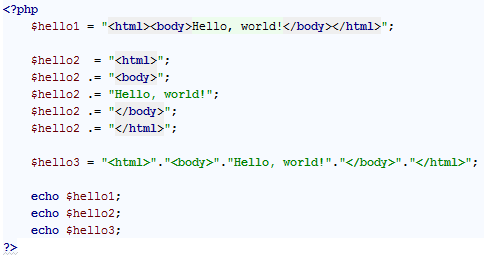
\includegraphics{Pictures/PHPStorm.PNG}
\caption{Пример поддержки встроенных языков в PHPStorm.}
\label{PHPStorm}
\end{figure}
}
\item
{
    IntelliLang \cite{IntelliLang} - плагин к средам разработки PHPStorm и IntelliJ IDEA \cite{IDEA}, c помощью которого для каждого строкового выражения можно указать, на каком языке оно написано. Например, IntelliLang для PHPStorm поддерживает различные диалекты языков запросов к базам данных. К недостаткам плагина следует отнести то, что для каждого строкового выражения нужно указывать язык явным образом.
}
\item
{
В статье Hyunha Kim, Kyung-Goo Doh and David Schmidt \cite{Kim} описан инструмент, осуществляющий статическую валидацию HTML-страниц, которые порождаются программами на PHP и JSP. К достоинствам инструмента является то, что валидация осуществляется как синтаксическая, так и семантическая. К примеру, этот инструмент может указывать на такие ошибки, как отсутствие обязательного атрибута, наличие двух разных элементов с одинаковым id и другие.
}
\item
{
    Alvor ~\cite{Alvor} ~--- это плагин к среде разработки Eclipse, который проверяет корректность встроенных SQL-выражений в код на Java. Ищет динамические выражения на SQL и проверяет их на соответствие SQL-грамматике. В случае, когда SQL-запросы содержат синтаксические и семантические ошибки, Alvor подчёркивает соответствующие места в исходном коде и выводит информацию об ошибках до запуска программы. 
}
\item 
{
    Java String Analyzer ~\cite{JSA}~--- это инструмент для анализа формирования строковых выражений на Java. Для каждого такого выражения он строит конечный автомат, представляющий приближённое значение всех значений этого выражения, которые могут быть получены во время исполнения. 
}
\item
{
PHP String Analyzer ~\cite{PSA} ~--- это инструмент для статического анализа строк, порождаемых PHP. Он аппроксимирует значения таких строк контекстно-свободной грамматикой. Это может быть использовано, например, для валидации генерируемых программами на PHP Web-страниц. 
}
\end{itemize}

Все приведённые выше инструменты, за исключением PHPStorm, предназначены для валидации динамически формируемых выражений, но не решают задачи подсветки синтаксиса встроенных языков. PHPStorm и IntelliLang (как вместе, так и по отдельности) решают эту задачу, но не для всех языков. Хотелось бы получить инструмент, который может осуществлять подсветку синтаксиса произвольного встроенного языка, описанного грамматикой.

\subsection{Обзор используемых инструментов}
\subsubsection{YaccConstructor}
На кафедре системного программирования математико-механического факультета СПбГУ разрабатывается инструмент YaccConstructor ~\cite{YC_paper}~\cite{YC_site}, позволяющий создавать генераторы синтаксических анализаторов под .NET. Основным языком разработки является мультипарадигмальный язык F\# \cite{FSharp}. Этот инструмент имеет модульную структуру, которая позволяет создавать анализаторы с различными алгоритмами разбора. Один из таких модулей создан для работы со встроенными языками. В рамках этого модуля уже реализованы алгоритмы абстрактного лексического и синтаксического анализа. “Абстрактный анализ” ~\cite{ARNGLR} здесь означает, что в качестве входа анализатор принимает не линейный поток токенов, а некую структуру. 

\begin{figure}[h]
\centering
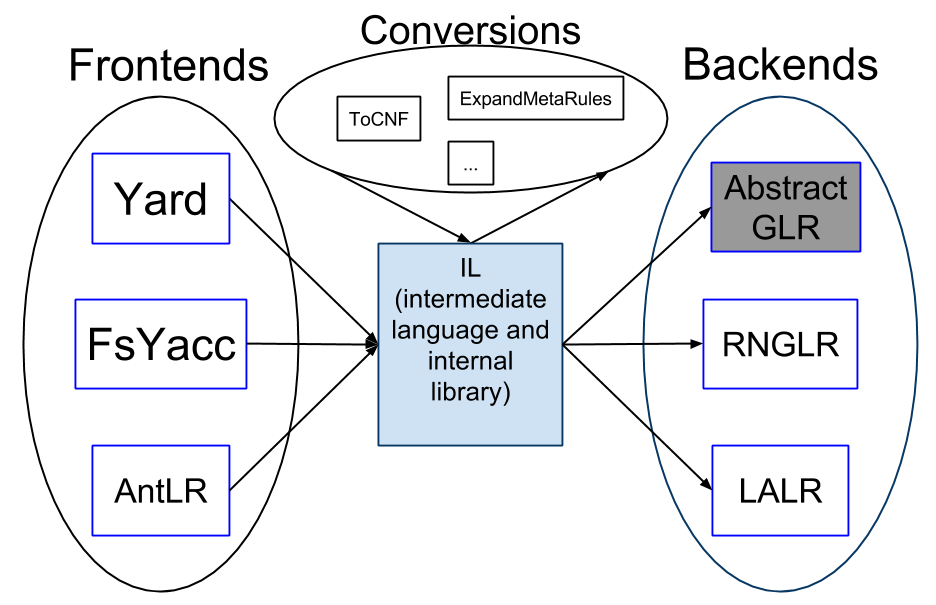
\includegraphics[width=100mm]{Pictures/YC_base.png}
\caption{Архитектура YaccConstructor}
\end{figure}

Рассмотрим работу абстрактного синтаксического анализатора чуть подробнее. 
\begin{itemize}
\item
{
На вход анализатору подаётся граф токенов (а не линейная последовательность, как в классическом анализе). Все токены образуют алгебраический тип данных Token, который создаётся генератором. Помимо этого каждый токен содержит в себе некоторую информацию: координаты в исходном файле (что необходимо при подсветке синтаксиса или же при уведомлении об ошибках).
}
\item
{По входному графу токенов строится SPPF ~\cite{RNGLR} (Shared Packed Parsed Forest) - структура, которая позволяет хранить все деревья разбора в сжатом виде. 
}
\item При необходимости можно осуществлять трансляцию деревьев. 
\end{itemize}
\subsubsection{ReSharper SDK}

Компания JetBrains разработала ReSharper - плагин к Microsoft Visual Studio, который позволяет повысить продуктивность работы, осуществляя дополнительные статические проверки и предоставляя дополнительные средства автодополнения, навигации, поиска и т.п.
У этого плагина есть свой SDK (Software Development Kit).  

Архитектура состоит из нескольких модулей. Рассмотрим некоторые из них.
\begin{itemize}
\item Platform - модуль, осуществляющий интеграцию с MS Visual Studio. Содержит в себе подмодули для работы с файлами solution, с файлами проектов, с файлами с исходным кодом. 

\item PSI (Project Structure Interface) - модуль, занимающийся структурой программы: лексический и синтаксический анализ языков, которые поддерживается ReSharper’ом. Содержит в себе компоненту, позволяющую добавлять поддержку новых языков. В данной работе используется PSI модуль используется для получения структуры программы на основном языке.

\item Daemon. Сборки Daemon являются работающими в фоновом режиме потоками, которые анализируют исходный код и реагируют на различные изменения в нём. 
	
\end{itemize}

При запуске программы ReSharper запускает свыше трёхсот сборок, которые осуществляют разнообразный анализ. Для того чтобы одна из этих сборок занималась каким-то самостоятельно реализованным анализом, нужно добавить какой-нибудь атрибут к определению класса (например, [DaemonStage] или [ContextAction]) и унаследоваться от какого-нибудь ReSharper’овского интерфейса (например, IDaemonStage). И тогда при запуске программы ReSharper инстанцирует требуемый класс и будет вызывать его методы при соответствующих изменениях. 

Тип этих изменений может определяться атрибутом. Например, класс, отмеченный атрибутом [DaemonStage], будет заново инстанцироваться при каждом изменении в файле с исходным кодом (например, напечатан или удалён какой-то символ). А если класс отмечен атрибутом [ContainsContextConsumer], то такая реакция будет происходить на каждое изменение положения курсора. 
